%
% Chapter 2 - Report Development
%
\chapter{Project development}

    This section describes the issues found and the decisions made
    to overcome them during development.

    \section{Relational database}

    Multiple iterations of the database's model were designed until a consistent result was implemented,
    mainly due to a lack of initial research on the project's functional requirements and a later change
    of some core beliefs regarding how meals would be handled.\\

    \section{Food API's}

    While testing an initial version of the HTTP server,
    it was concluded that no researched API responsible in
    providing accurate nutritional information exists.

    This conclusion came after comparing the nutritional values of multiple
    meals and ingredients from three APIs - Edamam, Nutrionix and Spoonacular -
    to the corresponding values provided by official portuguese sources. 
    The results can be found in [\nameref{app:nutritional_sheet}]

    We assumed that this inaccuracy is due to the fact that
    mentioned API's automatically calculate a recipe's carbohydrates
    from its ingredients without taking into consideration the cooking process, meaning that, for example,  
    100g of raw rice does not equal to the same amount of carbohydrates that 100g of 
    cooked rice might have.\\

    Another possible explanation is that there is no international standard for nutritional values,
    meaning that the same meal (and it's ingredients nutritional composition) 
    can have different carbohydrates between Portugal and the United States of America.\\
    
    As a result, the system no longer depends on food APIs meaning that every meal, ingredient and its' nutritional values
    need to be inserted manually by other sources, such as the developers themselves or authenticated users.
    For an initial release, we added around 60 basic ingredients and 30 meals.\\
    
    This comes with the limitation that certain ingredients might have been missed,
    meaning that a user might not be able to create their desired meals.

    \section{Android client}

    The Android application's development progressed normally but it had to be put on hold several times, because of HTTP server's endpoints' completion, in which the application
    depends strongly. A major dto and model restructure had also to be made inside the mobile application in order to meet with the current HTTP responses.\\

    \section{Restaurant APIs}

    During early stages of development, 
    we incorrectly assumed that researched restaurant APIs (namely Zomato) were capable 
    of providing menus for any restaurant in text form, and as such, their meals. Although such endpoint exists\cite{zomato}, 
    restaurant owners instead prefer to publish their menu as an image, 
    meaning that initially established functional requirements would never be able to be accomplished without 
    another viable alternative.\\

    As such, two alternatives were discussed:\\

    An OCR tool could be used in order to convert meals from a graphical menu to a text-based one.
    This implies additional response times for the user when querying a restaurant, due to the added layer 
    of communications and is not reliable in cases where restaurants
    design their menus with just an image of a meal and its' price.

    \begin{figure}[H]
        \begin{center}
            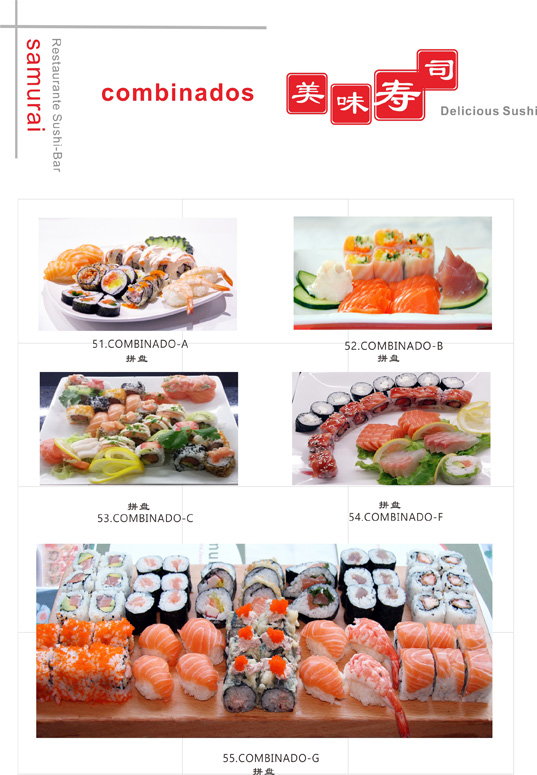
\includegraphics[scale=0.4]{_figures/examplemenu.jpg}
            \caption{An example of a restaurant's menu that would bring difficulties to the OCR translation}
        \end{center}
    \end{figure}

    Another alternative - and the adopted one - is to manually establish a set of statistically probable meals for cuisines
    and suggest them when obtaining a restaurant's information and cuisines.
    This solution is based on statistics and cultural assumptions meaning that not every suggestion might be accurate, which is
    why authenticated users' input is highly valuable in maintaining the system's data.\\